\documentclass[aspectratio=169,11pt]{beamer}

\usetheme{SimplePlus}

\usepackage{amsmath}
\usepackage{amssymb}
\usepackage{booktabs}
\usepackage{graphicx}
\usepackage{array}
\usepackage{tikz}
\usetikzlibrary{arrows.meta,positioning,calc}

\title{S181M116 Derivatives and Alternative Investments}
\subtitle{Lecture 5: Stochastic Calculus}
\author{Swapnil Singh}
\institute{Lietuvos Bankas and Kaunas University of Technology}
\date{}

\newcommand{\dt}{\Delta t}
\newcommand{\dz}{\Delta z}
\newcommand{\eps}{\varepsilon}
\newcommand{\E}{\mathbb{E}}
\newcommand{\Var}{\operatorname{Var}}
\newcommand{\Cov}{\operatorname{Cov}}
\newcommand{\Corr}{\operatorname{Corr}}
\newcommand{\Prob}{\mathbb{P}}
\newcommand{\Normal}{\mathcal{N}}
\newcommand{\given}{\,|\,}
\newcommand{\Szero}{S_0}
\newcommand{\St}{S_T}
\newcommand{\Ito}{Ito}

\AtBeginSection[]{
    \begin{frame}[plain,noframenumbering]
        \vfill
        \begin{center}
            {\usebeamerfont{subtitle}\usebeamercolor[fg]{structure}Section \thesection\par}
            \vspace{0.5em}
            {\usebeamerfont{title}\usebeamercolor[fg]{titlelike}\insertsectionhead\par}
        \end{center}

        \vspace{1.2em}
        \begin{center}
            \begin{minipage}{0.72\textwidth}
                \tableofcontents[currentsection,hideothersubsections]
            \end{minipage}
        \end{center}
        \vfill
    \end{frame}
}

\begin{document}

\begin{frame}
    \titlepage
\end{frame}

\begin{frame}{Today}
    \begin{enumerate}
        \item Why continuous-time derivative pricing needs stochastic processes.
        \item What the Markov property means for stock prices.
        \item How Brownian motion is built from independent normal increments.
        \item Why uncertainty scales with the square root of time.
        \item How drift and volatility enter a stochastic differential equation.
        \item Why stock prices are modeled with geometric Brownian motion.
        \item How to simulate stock price paths.
        \item How correlated shocks are constructed.
        \item Why stochastic calculus has different multiplication rules.
        \item How \Ito's lemma transforms functions of stochastic variables.
        \item Why geometric Brownian motion implies lognormal stock prices.
    \end{enumerate}
\end{frame}

\begin{frame}{Core Message}
    \begin{block}{The single most important scale difference}
        Ordinary calculus studies small changes of order \(dt\).
        Brownian shocks are of order \(\sqrt{dt}\):
        \[
            dz \approx \eps\sqrt{dt},
            \qquad
            \eps\sim\Normal(0,1).
        \]
    \end{block}

    \vspace{0.5em}
    \begin{alertblock}{Consequence}
        Since \((dz)^2\) is of order \(dt\), the square of a random shock does not disappear.
        This creates the extra \(\frac{1}{2}\) term in \Ito's lemma.
    \end{alertblock}
\end{frame}

\begin{frame}{From Binomial Trees to Brownian Motion}
    Lecture 4 used a binomial tree:
    \[
        S \rightarrow Su
        \quad \text{or} \quad
        S \rightarrow Sd.
    \]

    \vspace{0.4em}
    Continuous-time finance asks what happens as:
    \begin{itemize}
        \item the number of steps becomes very large;
        \item each time step becomes very small;
        \item the up/down random walk converges to a continuous random path.
    \end{itemize}

    \begin{block}{Bridge}
        Brownian motion is the continuous-time limit object behind many recombining tree models.
        It lets us do local hedging and obtain differential equations.
    \end{block}
\end{frame}



\begin{frame}{One Stock Path, Finer Observation Intervals}
	\small
	\begin{center}
		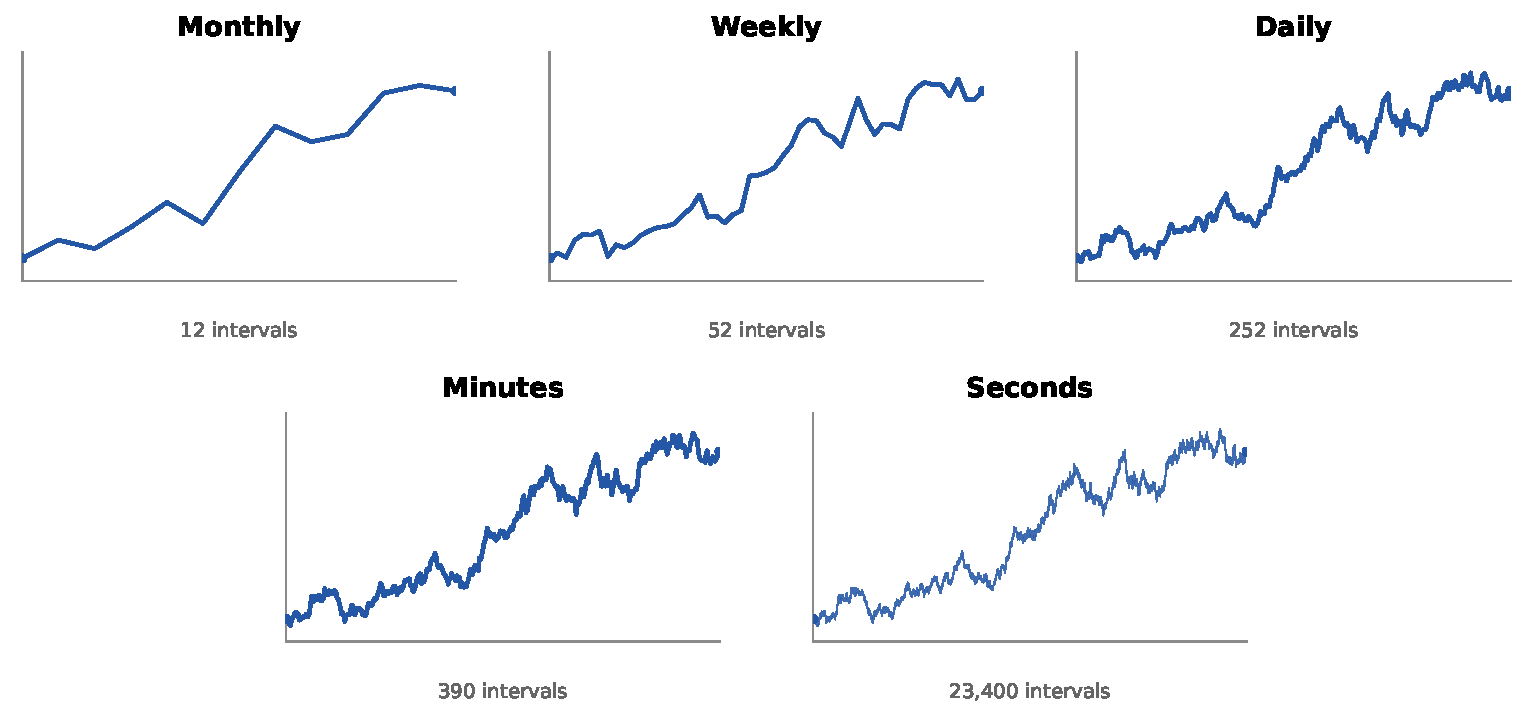
\includegraphics[width=0.92\textwidth,height=0.58\textheight,keepaspectratio]{images/stock-frequency-sampling.pdf}
	\end{center}
	
	\vspace{-0.2em}
	\begin{block}{Intuition}
		As the observation interval \(\dt\) shrinks, each move is smaller but there are many more moves.
		The limiting object is a continuous but jagged random path, not an ordinary differentiable curve.
	\end{block}
\end{frame}


\section{Stochastic Processes}

\begin{frame}{What Is a Stochastic Process?}
    \begin{block}{Definition}
        A stochastic process is a collection of random variables indexed by time:
        \[
            \{X_t: t\geq 0\}.
        \]
        Each \(X_t\) is the uncertain value of the variable at date \(t\).
    \end{block}

    \begin{columns}[T]
        \begin{column}{0.48\textwidth}
            \begin{block}{Time}
                \begin{itemize}
                    \item Discrete time: \(t=0,1,2,\ldots\).
                    \item Continuous time: \(t\in[0,T]\).
                \end{itemize}
            \end{block}
        \end{column}
        \begin{column}{0.48\textwidth}
            \begin{block}{State}
                \begin{itemize}
                    \item Discrete state: finite/countable values.
                    \item Continuous state: any value in an interval.
                \end{itemize}
            \end{block}
        \end{column}
    \end{columns}
\end{frame}

\begin{frame}{Four Types of Processes}
    \begin{center}
    \begin{tabular}{lll}
        \toprule
        & \textbf{Discrete state} & \textbf{Continuous state} \\
        \midrule
        \textbf{Discrete time}
        & Binomial tree
        & AR(1) return model \\
        \textbf{Continuous time}
        & Poisson jump process
        & Brownian stock model \\
        \bottomrule
    \end{tabular}
    \end{center}

    \vspace{1em}
    \begin{alertblock}{Model versus reality}
        Real stock prices trade in ticks and only when markets are open.
        Continuous-time models are approximations chosen because they are tractable and useful.
    \end{alertblock}
\end{frame}

\begin{frame}[label=markov_main]{The Markov Property}
    \begin{block}{Definition}
        The future depends on the current state, not on the path taken to reach it:
        \[
            \Prob(X_u\leq x\given X_t,X_{t_1},\ldots,X_{t_n})
            =
            \Prob(X_u\leq x\given X_t),
            \qquad t_i<t<u.
        \]
    \end{block}

    \begin{exampleblock}{Stock price interpretation}
        If the stock price is 100 today, the model's future distribution depends on 100 and current parameters.
        It does not separately depend on whether the stock was 80 or 120 last month.
    \end{exampleblock}

    \hyperlink{deriv_markov}{\beamergotobutton{Conditional-distribution detail}}
\end{frame}

\begin{frame}{Markov Does Not Mean History Is Useless}
    \begin{columns}[T]
        \begin{column}{0.48\textwidth}
            \begin{block}{History can help estimate}
                \begin{itemize}
                    \item volatility;
                    \item jump frequency;
                    \item correlations;
                    \item time-varying parameters.
                \end{itemize}
            \end{block}
        \end{column}
        \begin{column}{0.48\textwidth}
            \begin{block}{Markov means}
                After parameters and current state are known, the past path is not an additional state variable.
            \end{block}

            \begin{alertblock}{Market-efficiency intuition}
                Predictable patterns in past prices tend to be traded away.
            \end{alertblock}
        \end{column}
    \end{columns}
\end{frame}

\section{Brownian Motion}

\begin{frame}[label=variance_scaling_main]{Variance and the Square Root of Time}
    Suppose independent one-year changes satisfy
    \[
        \Delta X_1\sim\Normal(0,1).
    \]

    For two years, the total change is the sum of two independent one-year changes:
    \[
        \Delta X_{\text{2 years}}
        =
        \Delta X_{\text{year 1}}
        +
        \Delta X_{\text{year 2}},
        \qquad
        \Delta X_{\text{year 1}},\Delta X_{\text{year 2}}
        \sim\Normal(0,1).
    \]

    \begin{block}{Key rule}
        Means add and variances add:
        \[
            \Delta X_{\text{2 years}}\sim\Normal(0,2),
            \qquad
            \operatorname{sd}(\Delta X_{\text{2 years}})=\sqrt{2}.
        \]
    \end{block}

    \hyperlink{deriv_variance_scaling}{\beamergotobutton{Derive variance scaling}}
\end{frame}

\begin{frame}{Volatility Scaling Example}
    \small
    Annual volatility of \(20\%\) means a one-year return has standard deviation \(20\%\).
    Shorter horizons have less uncertainty because fewer shocks have accumulated.

    \begin{block}{Rule}
        \[
            \sigma_{\text{horizon}}
            =
            \sigma_{\text{annual}}\sqrt{\text{fraction of a year}}
        \]
    \end{block}

    \begin{center}
        \footnotesize
        \begin{tabular}{lcc}
            \toprule
            Horizon & Fraction of year & One-standard-deviation move \\
            \midrule
            1 year  & \(1\)          & \(20.00\%\) \\
            1 month & \(1/12\)       & \(20\%\sqrt{1/12}=5.77\%\) \\
            1 week  & \(1/52\)       & \(20\%\sqrt{1/52}=2.77\%\) \\
            1 day   & \(1/252\)      & \(20\%\sqrt{1/252}=1.26\%\) \\
            \bottomrule
        \end{tabular}
    \end{center}

    \begin{alertblock}{Common mistake}
        Divide monthly volatility by \(\sqrt{12}\), not by \(12\).
        Variance scales linearly with time; volatility scales with \(\sqrt{\text{time}}\).
    \end{alertblock}
\end{frame}

\begin{frame}{Wiener Process}
    \begin{block}{Definition}
        A process \(z_t\) is a Wiener process, or standard Brownian motion, if:
        \begin{enumerate}
            \item over a small interval \(\dt\),
            \[
                \dz=\eps\sqrt{\dt},
                \qquad
                \eps\sim\Normal(0,1);
            \]
            \item increments over non-overlapping intervals are independent.
        \end{enumerate}
    \end{block}

    Hence:
    \[
        \E[\dz]=0,
        \qquad
        \Var(\dz)=\dt,
        \qquad
        z_T-z_0\sim\Normal(0,T).
    \]
\end{frame}

\begin{frame}{Brownian Motion as a Limit}
    \begin{center}
        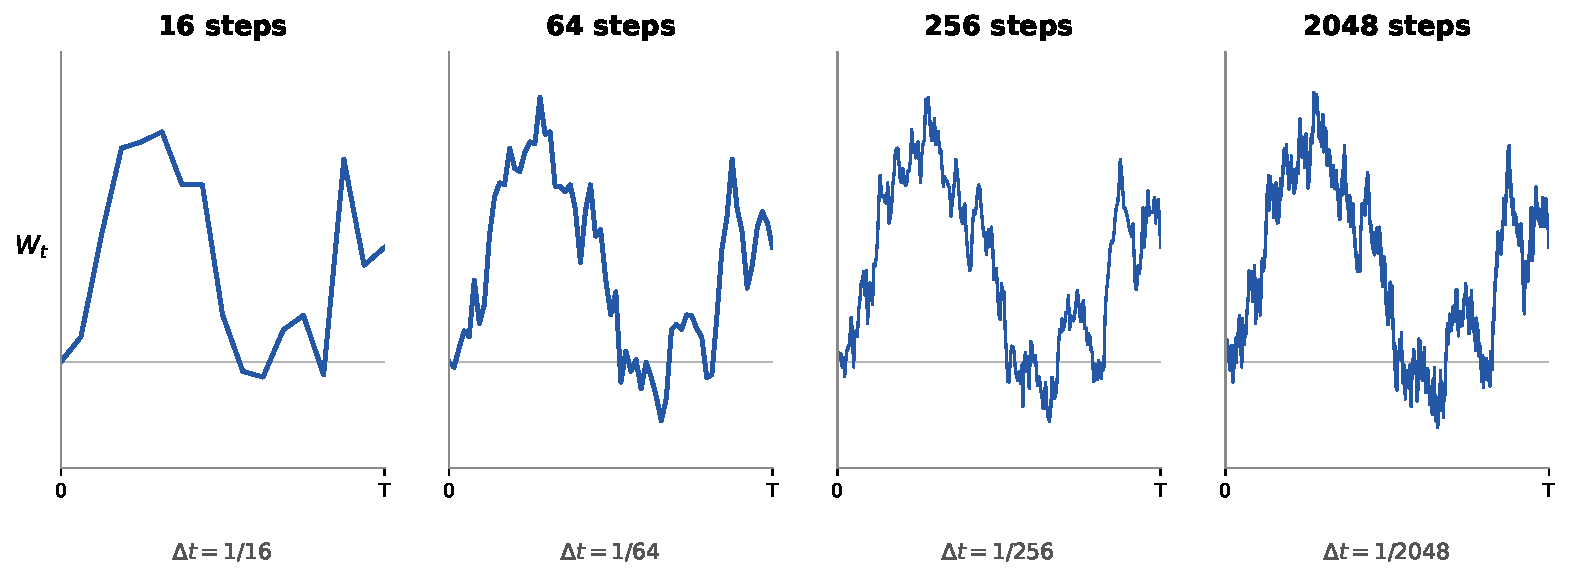
\includegraphics[width=0.96\textwidth,height=0.58\textheight,keepaspectratio]{images/brownian-motion-limit.pdf}
    \end{center}

    \begin{block}{Path intuition}
        Brownian motion is continuous, but not smooth.
        It has no ordinary instantaneous slope because smaller time grids keep revealing new variation.
    \end{block}
\end{frame}


\section{Drift, Volatility, and Stock Prices}

\begin{frame}{Generalized Wiener Process}
    A standard Wiener process has zero drift and variance rate one.

    \begin{block}{Add drift and scale}
        \[
            dx=a\,dt+b\,dz.
        \]
    \end{block}

    Over a small interval:
    \[
        \Delta x=a\dt+b\eps\sqrt{\dt}.
    \]

    Therefore:
    \[
        \E[\Delta x]=a\dt,
        \qquad
        \Var(\Delta x)=b^2\dt.
    \]
\end{frame}


\begin{frame}{Adding Drift and Volatility}
	\begin{center}
		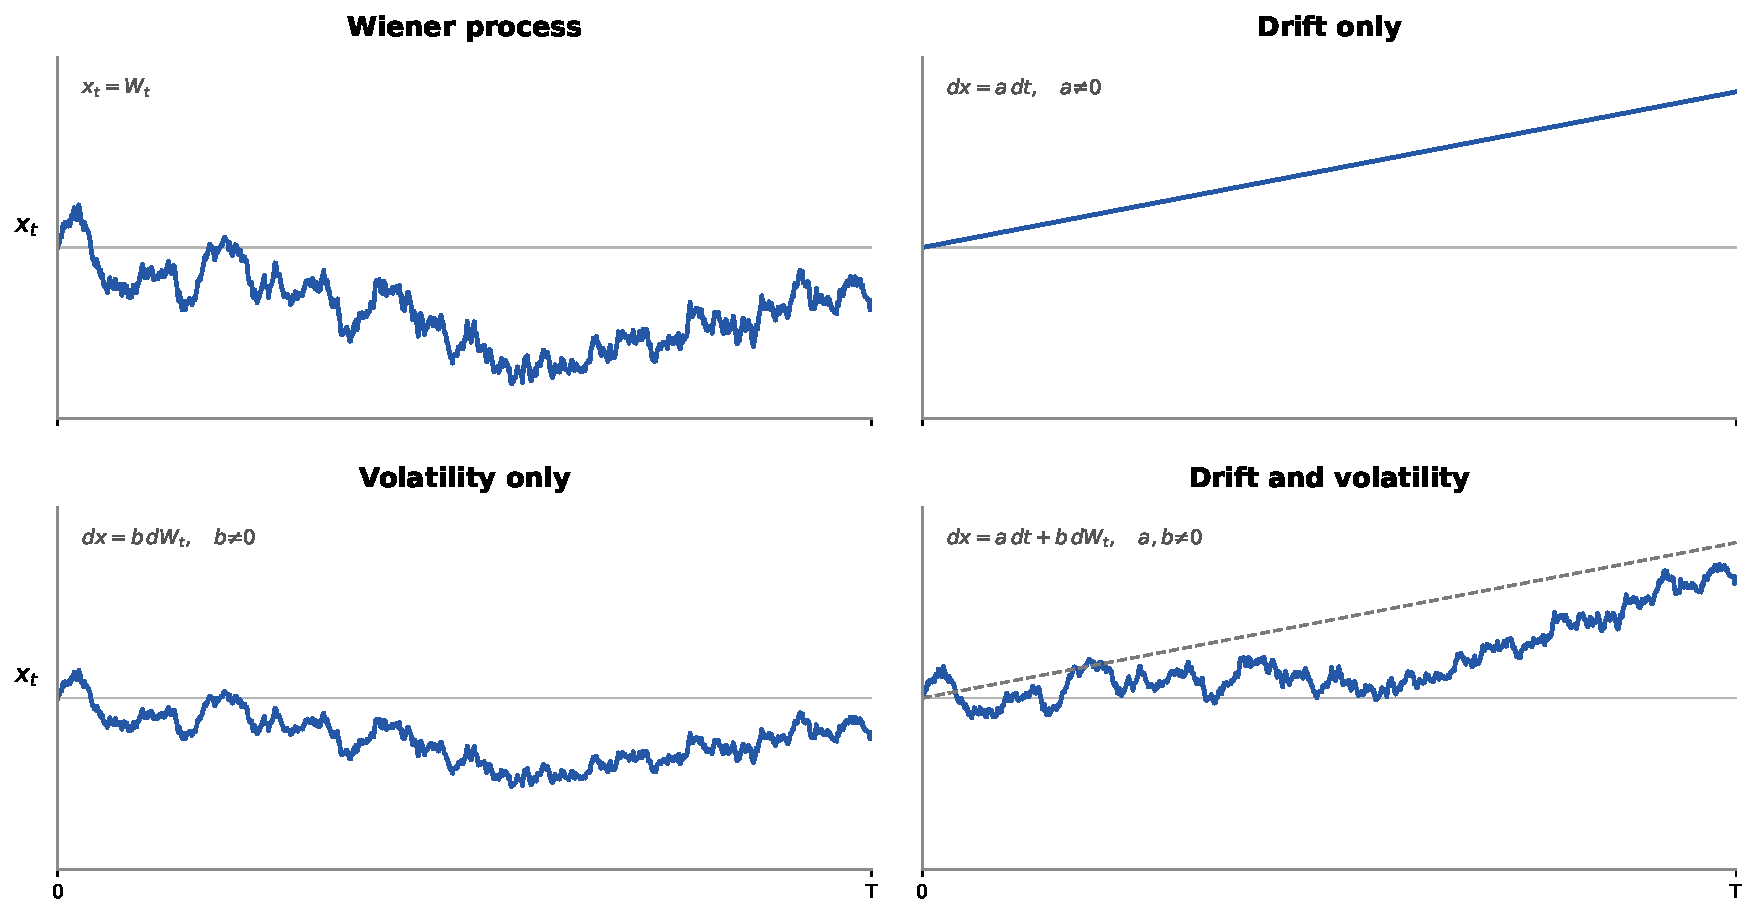
\includegraphics[width=0.96\textwidth,height=0.78\textheight,keepaspectratio]{images/wiener-drift-volatility.pdf}
	\end{center}
\end{frame}

\begin{frame}{Why Brownian Paths Are Jagged}
	Brownian increments satisfy
	\[
	dz \approx \eps\sqrt{dt}.
	\]
	
	For small \(dt\), \(\sqrt{dt}\) is much larger than \(dt\):
	\[
	dt=0.0001
	\quad \Rightarrow \quad
	\sqrt{dt}=0.01.
	\]
	
	\begin{alertblock}{Implication}
		Random movement dominates deterministic drift at very short horizons.
		This makes Brownian paths locally rough rather than tangent-line smooth.
	\end{alertblock}
\end{frame}

\begin{frame}{Drift and Volatility: Visual Interpretation}
    \begin{columns}[T]
        \begin{column}{0.48\textwidth}
            \begin{block}{Drift \(a\)}
                Moves the center of the distribution:
                \[
                    \E[x_T-x_0]=aT.
                \]
            \end{block}
        \end{column}
        \begin{column}{0.48\textwidth}
            \begin{block}{Diffusion coefficient \(b\)}
                Controls dispersion:
                \[
                    \operatorname{sd}(x_T-x_0)=b\sqrt{T}.
                \]
            \end{block}
        \end{column}
    \end{columns}

    \vspace{0.8em}
    \begin{alertblock}{Mental model}
        Drift moves the center of the cloud.
        Volatility changes the width of the cloud.
        A single path can still move against the drift.
    \end{alertblock}
\end{frame}

\begin{frame}{Numerical Example: Cash Balance}
    Cash balance, in thousands, follows
    \[
        dx=20\,dt+30\,dz.
    \]

    If \(x_0=50\), then after one year:
    \[
        x_1\sim\Normal(70,900),
        \qquad
        \operatorname{sd}(x_1)=30.
    \]

    After six months:
    \[
        x_{0.5}\sim\Normal(60,450),
        \qquad
        \operatorname{sd}(x_{0.5})=21.21.
    \]

    \begin{block}{Interpretation}
        The mean moves linearly with time.
        The standard deviation moves with \(\sqrt{T}\).
    \end{block}
\end{frame}

\begin{frame}{Ito Process}
    A generalized Wiener process uses constant \(a\) and \(b\).

    \begin{block}{State-dependent drift and volatility}
        \[
            dx=a(x,t)\,dt+b(x,t)\,dz.
        \]
    \end{block}

    Over a small interval:
    \[
        \Delta x
        \approx
        a(x,t)\dt+b(x,t)\eps\sqrt{\dt}.
    \]

    \begin{alertblock}{Local approximation}
        In the next instant, evaluate drift and volatility at the current state \((x,t)\).
        Then update the state and repeat.
    \end{alertblock}
\end{frame}

\begin{frame}{Why Stock Prices Need Percentage Shocks}
    \footnotesize
    Stock investors care about \emph{returns}, not raw dollar moves:
    \[
        \text{return}=\frac{\Delta S}{S}.
    \]

    \begin{columns}[T]
        \begin{column}{0.48\textwidth}
            \begin{alertblock}{Constant dollar shock}
                \centering
                \(dS=a\,dt+b\,dz\)

                \vspace{0.25em}
                Same dollar shock, different return.

                \vspace{0.25em}
                \begin{tabular}{lcc}
                    \toprule
                    Price & Shock & Return \\
                    \midrule
                    \(\$10\)  & \(\$2\) & \(20\%\) \\
                    \(\$200\) & \(\$2\) & \(1\%\) \\
                    \bottomrule
                \end{tabular}
            \end{alertblock}
        \end{column}
        \begin{column}{0.48\textwidth}
            \begin{block}{Percentage shock}
                \centering
                \(\frac{dS}{S}=\mu\,dt+\sigma\,dz\)

                \vspace{0.25em}
                Same return shock, different dollar move.

                \vspace{0.25em}
                \begin{tabular}{lcc}
                    \toprule
                    Price & Shock & Return \\
                    \midrule
                    \(\$10\)  & \(\$0.20\) & \(2\%\) \\
                    \(\$200\) & \(\$4.00\) & \(2\%\) \\
                    \bottomrule
                \end{tabular}
            \end{block}
        \end{column}
    \end{columns}

    \vspace{0.35em}
    \begin{center}
        \(\Delta S = S\times \text{return shock}\)
        \qquad \(\Longrightarrow\qquad\)
        \(dS=\mu S\,dt+\sigma S\,dz\).
    \end{center}
\end{frame}

\begin{frame}[label=gbm_main]{Geometric Brownian Motion}
    \begin{block}{Stock price model}
        \[
            dS=\mu S\,dt+\sigma S\,dz,
            \qquad
            \frac{dS}{S}=\mu\,dt+\sigma\,dz.
        \]
    \end{block}

    \begin{columns}[T]
        \begin{column}{0.48\textwidth}
            \begin{block}{\(\mu\)}
                Real-world expected continuously compounded return.
            \end{block}
        \end{column}
        \begin{column}{0.48\textwidth}
            \begin{block}{\(\sigma\)}
                Volatility: standard deviation of log returns per square root of year.
            \end{block}
        \end{column}
    \end{columns}

    \vspace{0.5em}
    \hyperlink{deriv_gbm_no_uncertainty}{\beamergotobutton{Deterministic growth derivation}}
\end{frame}

\begin{frame}{Discrete-Time Approximation}
    From
    \[
        \frac{dS}{S}=\mu\,dt+\sigma\,dz,
    \]
    the small-step approximation is
    \[
        \frac{\Delta S}{S}
        =
        \mu\dt+\sigma\eps\sqrt{\dt}.
    \]

    Therefore, approximately:
    \[
        \frac{\Delta S}{S}
        \sim
        \Normal(\mu\dt,\sigma^2\dt).
    \]

    \begin{block}{Interpretation}
        Expected return over \(\dt\) is \(\mu\dt\).
        Return standard deviation over \(\dt\) is \(\sigma\sqrt{\dt}\).
    \end{block}
\end{frame}

\begin{frame}{Weekly Return Example}
    Let
    \[
        \mu=15\%,
        \qquad
        \sigma=30\%,
        \qquad
        \dt=\frac{1}{52}=0.01923.
    \]

    Then
    \[
        \frac{\Delta S}{S}
        =
        0.15(0.01923)+0.30\eps\sqrt{0.01923}
        =
        0.00288+0.0416\eps.
    \]

    \begin{exampleblock}{Interpretation}
        Expected weekly return is \(0.288\%\).
        Weekly return standard deviation is \(4.16\%\).
    \end{exampleblock}
\end{frame}

\section{Simulation and Correlation}

\begin{frame}{Euler Simulation of GBM}
    The simple simulation update is
    \[
        S_{t+\dt}
        =
        S_t\left(1+\mu\dt+\sigma\eps\sqrt{\dt}\right).
    \]

    \begin{enumerate}
        \item Choose a time step \(\dt\).
        \item Draw \(\eps\sim\Normal(0,1)\).
        \item Update \(S\).
        \item Repeat with independent new shocks.
    \end{enumerate}

    \begin{alertblock}{Important}
        This is an approximation. For GBM there is also an exact lognormal update.
    \end{alertblock}
\end{frame}

\begin{frame}[label=lognormal_sim_main]{Exact Lognormal Simulation}
    For geometric Brownian motion with constant \(\mu\) and \(\sigma\):
    \[
        S_{t+\dt}
        =
        S_t
        \exp\left[
            \left(\mu-\frac{1}{2}\sigma^2\right)\dt
            +
            \sigma\sqrt{\dt}\eps
        \right].
    \]

    \begin{block}{Why use this?}
        \begin{itemize}
            \item It keeps prices positive.
            \item It is exact for GBM.
            \item It follows from applying \Ito's lemma to \(\ln S\).
        \end{itemize}
    \end{block}

    \hyperlink{deriv_lognormal}{\beamergotobutton{Derive lognormal update}}
\end{frame}

\begin{frame}{One Simulated Step}
    Let
    \[
        S_t=100,\quad
        \mu=0.15,\quad
        \sigma=0.30,\quad
        \dt=\frac{1}{52},\quad
        \eps=0.52.
    \]

    Euler gives
    \[
        \Delta S
        =
        100(0.00288+0.0416(0.52))
        =
        2.45.
    \]

    The next simulated price is
    \[
        S_{t+\dt}=102.45.
    \]
\end{frame}

\begin{frame}{Annualizing Volatility}
    If \(\sigma\) is annual volatility, return standard deviation over \(T\) years is
    \[
        \sigma\sqrt{T}.
    \]

    With 252 trading days:
    \[
        \sigma_{\text{daily}}
        =
        \frac{\sigma_{\text{annual}}}{\sqrt{252}},
        \qquad
        \sigma_{\text{annual}}
        =
        \sigma_{\text{daily}}\sqrt{252}.
    \]

    \begin{exampleblock}{Example}
        Annual volatility \(32\%\) implies daily volatility
        \[
            \frac{0.32}{\sqrt{252}}=2.02\%.
        \]
    \end{exampleblock}
\end{frame}

\begin{frame}[label=correlation_main]{Correlated Wiener Processes}
    Suppose
    \[
        dx_1=a_1dt+b_1dz_1,
        \qquad
        dx_2=a_2dt+b_2dz_2.
    \]

    If the Brownian shocks have correlation \(\rho\), we write:
    \[
        \Corr(dz_1,dz_2)=\rho,
        \qquad
        dz_1dz_2=\rho\,dt.
    \]

    \begin{block}{Financial uses}
        Multi-asset options, spread options, stochastic volatility models, interest-rate models, and risk simulations.
    \end{block}

    \hyperlink{deriv_correlated_normals}{\beamergotobutton{Construct correlated normals}}
\end{frame}

\begin{frame}{Example: Correlated Shocks}
    Draw independent \(u,v\sim\Normal(0,1)\) and set
    \[
        \eps_1=u,
        \qquad
        \eps_2=\rho u+\sqrt{1-\rho^2}\,v.
    \]

    If \(\rho=0.60\), \(u=1.10\), and \(v=-0.40\), then:
    \[
        \eps_1=1.10,
        \qquad
        \eps_2=0.60(1.10)+0.80(-0.40)=0.34.
    \]

    \begin{block}{Interpretation}
        \(\eps_2\) has a common component with \(\eps_1\) plus independent residual noise.
    \end{block}
\end{frame}

\section{Stochastic Calculus}

\begin{frame}[label=quadvar_main]{The Multiplication Rules}
    Since
    \[
        dz\approx \eps\sqrt{dt},
    \]
    we use the informal table:
    \[
        (dt)^2=0,
        \qquad
        dt\,dz=0,
        \qquad
        (dz)^2=dt.
    \]

    For correlated Brownian motions:
    \[
        dz_i dz_j=\rho_{ij}dt.
    \]

    \begin{alertblock}{Key intuition}
        The square of the Brownian shock survives because it is order \(dt\).
    \end{alertblock}

    \hyperlink{deriv_quadratic_variation}{\beamergotobutton{Why \((dz)^2=dt\)?}}
\end{frame}

\begin{frame}[label=ito_statement]{Ito's Lemma}
    Let
    \[
        dx=a(x,t)dt+b(x,t)dz,
        \qquad
        G=G(x,t).
    \]

    Then
    \[
        dG
        =
        \left(
            G_xa+G_t+\frac{1}{2}G_{xx}b^2
        \right)dt
        +
        G_xb\,dz.
    \]

    \begin{alertblock}{Compared with ordinary calculus}
        The extra term is
        \[
            \frac{1}{2}G_{xx}b^2dt.
        \]
        It comes from curvature times variance.
    \end{alertblock}

    \hyperlink{deriv_ito}{\beamergotobutton{Derive Ito's lemma}}
\end{frame}

\begin{frame}{Financial Interpretation of Ito's Lemma}
    Let \(G(S,t)\) be an option value and \(S\) the underlying stock.

    \[
        dG
        =
        \left(
            G_S\mu S+G_t+\frac{1}{2}G_{SS}\sigma^2S^2
        \right)dt
        +
        G_S\sigma S\,dz.
    \]

    \begin{columns}[T]
        \begin{column}{0.32\textwidth}
            \begin{block}{Delta}
                \(G_S\): first-order exposure to the stock.
            \end{block}
        \end{column}
        \begin{column}{0.32\textwidth}
            \begin{block}{Theta}
                \(G_t\): direct effect of time passing.
            \end{block}
        \end{column}
        \begin{column}{0.32\textwidth}
            \begin{block}{Gamma}
                \(G_{SS}\): curvature interacting with variance.
            \end{block}
        \end{column}
    \end{columns}
\end{frame}

\begin{frame}[label=ito_examples_main]{Example: Squaring Brownian Motion}
    Let \(x=z\), so \(dx=dz\), and take
    \[
        G(x)=x^2.
    \]

    Since
    \[
        G_x=2x,
        \qquad
        G_{xx}=2,
    \]
    \Ito's lemma gives
    \[
        d(x^2)=2x\,dz+dt.
    \]

    \begin{alertblock}{Ordinary calculus would miss the \(dt\) term}
        The extra \(dt\) is accumulated Brownian variance.
    \end{alertblock}

    \hyperlink{deriv_power}{\beamergotobutton{Power-function example}}
\end{frame}

\begin{frame}[label=forward_main]{Application: Forward Price Dynamics}
    For a non-dividend-paying stock and constant \(r\), the forward price at time \(t\) for maturity \(T\) is
    \[
        F(S,t)=S e^{r(T-t)}.
    \]

    If
    \[
        dS=\mu Sdt+\sigma Sdz,
    \]
    then \Ito's lemma gives
    \[
        dF=(\mu-r)Fdt+\sigma Fdz.
    \]

    \begin{block}{Interpretation}
        The forward price has the same volatility as the stock and real-world drift \(\mu-r\).
    \end{block}

    \hyperlink{deriv_forward}{\beamergotobutton{Derive forward dynamics}}
\end{frame}

\section{Lognormal Stock Prices}

\begin{frame}[label=log_process_main]{Applying Ito to \(\ln S\)}
    If
    \[
        \frac{dS}{S}=\mu dt+\sigma dz,
    \]
    then applying \Ito's lemma to \(G(S)=\ln S\) gives
    \[
        d\ln S
        =
        \left(\mu-\frac{1}{2}\sigma^2\right)dt+\sigma dz.
    \]

    \begin{alertblock}{Ito correction}
        Expected log growth is lower than expected arithmetic instantaneous return by
        \[
            \frac{1}{2}\sigma^2.
        \]
    \end{alertblock}

    \hyperlink{deriv_log_process}{\beamergotobutton{Derive \(d\ln S\)}}
\end{frame}

\begin{frame}{Why Volatility Lowers Log Growth}
    Equal percentage gains and losses do not offset in compounded wealth.

    \begin{exampleblock}{Simple arithmetic}
        A 50\% gain followed by a 50\% loss:
        \[
            100 \rightarrow 150 \rightarrow 75.
        \]
        The arithmetic average return is zero, but wealth falls.
    \end{exampleblock}

    \begin{block}{Continuous-time version}
        The correction \(-\frac{1}{2}\sigma^2\) captures this compounding effect in the GBM model.
    \end{block}
\end{frame}

\begin{frame}[label=terminal_distribution_main]{Terminal Distribution}
    Integrating
    \[
        d\ln S
        =
        \left(\mu-\frac{1}{2}\sigma^2\right)dt+\sigma dz
    \]
    from 0 to \(T\):
    \[
        \ln S_T
        \sim
        \Normal\left(
            \ln S_0+\left(\mu-\frac{1}{2}\sigma^2\right)T,
            \sigma^2T
        \right).
    \]

    \begin{alertblock}{Conclusion}
        \(S_T\) is lognormally distributed.
        Log prices are normal; prices are positive and right-skewed.
    \end{alertblock}

    \hyperlink{deriv_lognormal}{\beamergotobutton{Distribution derivation}}
\end{frame}

\begin{frame}{Mean versus Median}
    Under real-world GBM:
    \[
        \E[S_T]=S_0e^{\mu T}.
    \]

    The median is
    \[
        \operatorname{median}(S_T)
        =
        S_0e^{(\mu-\frac{1}{2}\sigma^2)T}.
    \]

    \begin{block}{Why they differ}
        The lognormal distribution is right-skewed.
        Rare large upward outcomes raise the mean above the median.
    \end{block}
\end{frame}

\begin{frame}{Numerical Distribution Example}
    Let
    \[
        S_0=100,\qquad
        \mu=12\%,\qquad
        \sigma=30\%,\qquad
        T=1.
    \]

    Then
    \[
        \ln S_1
        \sim
        \Normal(\ln 100+0.075,0.09).
    \]

    \begin{columns}[T]
        \begin{column}{0.48\textwidth}
            \[
                \E[S_1]=100e^{0.12}=112.75.
            \]
        \end{column}
        \begin{column}{0.48\textwidth}
            \[
                \operatorname{median}(S_1)=100e^{0.075}=107.79.
            \]
        \end{column}
    \end{columns}
\end{frame}

\begin{frame}[label=risk_neutral_preview_main]{Preview: Risk-Neutral Dynamics}
    Real-world stock dynamics:
    \[
        \frac{dS}{S}=\mu dt+\sigma dz.
    \]

    Risk-neutral stock dynamics for a non-dividend-paying stock:
    \[
        \frac{dS}{S}=r dt+\sigma dz^Q.
    \]

    \begin{alertblock}{Pricing lesson for Lecture 6}
        In Black-Scholes-Merton, the real-world expected return \(\mu\) does not enter the option price.
        Dynamic hedging replaces it with the risk-free rate \(r\).
    \end{alertblock}

    \hyperlink{deriv_risk_neutral_distribution}{\beamergotobutton{Risk-neutral terminal distribution}}
\end{frame}

\begin{frame}{Where We Are Going Next}
    Lecture 6 uses today's machinery to price options.

    \begin{enumerate}
        \item Use \Ito's lemma for an option value \(V(S,t)\).
        \item Combine the option and stock to eliminate the \(dz\) risk.
        \item The locally riskless portfolio must earn \(r\).
        \item This gives the Black-Scholes-Merton PDE.
        \item Solve the PDE or use risk-neutral valuation to get option formulas.
    \end{enumerate}

    \begin{block}{Key bridge}
        The common Brownian shock in \(dS\) and \(dV\) is what makes delta hedging possible.
    \end{block}
\end{frame}

\begin{frame}{Checklist}
    After this lecture you should be able to:
    \begin{itemize}
        \item define stochastic process, Markov process, and Wiener process;
        \item explain square-root-time volatility scaling;
        \item write generalized Wiener, \Ito, and GBM processes;
        \item simulate a GBM step and annualize volatility;
        \item construct correlated normal shocks;
        \item use the stochastic multiplication table;
        \item state and apply \Ito's lemma;
        \item derive \(d\ln S\) from GBM;
        \item state the lognormal distribution of \(S_T\);
        \item explain the real-world versus risk-neutral drift change.
    \end{itemize}
\end{frame}

\begin{frame}{Practice Questions}
    \begin{enumerate}
        \item If annual volatility is \(24\%\), what is one-month volatility?
        \item If \(z_t\) is Brownian motion, what is the distribution of \(z_3-z_1\)?
        \item For \(dx=5dt+2dz\), find the mean and variance of \(x_T-x_0\).
        \item For \(dS/S=0.10dt+0.25dz\), find the approximate one-week return distribution.
        \item Use \Ito's lemma to find \(d(S^2)\) when \(dS=\mu Sdt+\sigma Sdz\).
        \item Derive \(d\ln S\) and explain the \(-\sigma^2/2\) term.
        \item State the distribution of \(\ln S_T\) under risk-neutral dynamics.
    \end{enumerate}
\end{frame}

\appendix
\section{Appendix Derivations}

\begin{frame}[label=deriv_markov]{Appendix: Markov Conditional Distribution}
    A process is Markov if the current state is a sufficient statistic for the future:
    \[
        \Prob(X_u\in A \given \mathcal{F}_t)
        =
        \Prob(X_u\in A \given X_t),
        \qquad u>t.
    \]

    Here \(\mathcal{F}_t\) means all information generated by the process up to time \(t\).

    \begin{block}{Implication}
        If two histories reach the same current value \(X_t=x\), the model assigns the same future distribution to both histories.
    \end{block}

    \hyperlink{markov_main}{\beamerreturnbutton{Back to Markov slide}}
\end{frame}

\begin{frame}[label=deriv_variance_scaling]{Appendix: Variance Scaling}
    Let the change over \(T\) be divided into \(N\) independent increments:
    \[
        \Delta X_T=\sum_{i=1}^N \Delta X_i,
        \qquad
        \Delta X_i\sim\Normal(0,\dt),
        \qquad
        N\dt=T.
    \]

    Then
    \[
        \E[\Delta X_T]
        =
        \sum_{i=1}^N \E[\Delta X_i]
        =
        0,
    \]
    and independence gives
    \[
        \Var(\Delta X_T)
        =
        \sum_{i=1}^N \Var(\Delta X_i)
        =
        N\dt=T.
    \]

    Therefore \(\operatorname{sd}(\Delta X_T)=\sqrt{T}\).

    \hyperlink{variance_scaling_main}{\beamerreturnbutton{Back to variance slide}}
\end{frame}

\begin{frame}[label=deriv_gbm_no_uncertainty]{Appendix: Deterministic Growth}
    If there is no uncertainty in GBM,
    \[
        dS=\mu Sdt.
    \]

    Divide by \(S\):
    \[
        \frac{dS}{S}=\mu dt.
    \]

    Integrate from 0 to \(T\):
    \[
        \int_{S_0}^{S_T}\frac{dS}{S}
        =
        \int_0^T \mu dt.
    \]

    Hence
    \[
        \ln S_T-\ln S_0=\mu T,
        \qquad
        S_T=S_0e^{\mu T}.
    \]

    \hyperlink{gbm_main}{\beamerreturnbutton{Back to GBM slide}}
\end{frame}

\begin{frame}[label=deriv_correlated_normals]{Appendix: Correlated Normal Construction}
    Draw independent \(u,v\sim\Normal(0,1)\). Define
    \[
        \eps_1=u,
        \qquad
        \eps_2=\rho u+\sqrt{1-\rho^2}v.
    \]

    Means:
    \[
        \E[\eps_1]=0,
        \qquad
        \E[\eps_2]=0.
    \]

    Variance of \(\eps_2\):
    \[
        \Var(\eps_2)=\rho^2\Var(u)+(1-\rho^2)\Var(v)=1.
    \]

    Covariance:
    \[
        \Cov(\eps_1,\eps_2)
        =
        \Cov(u,\rho u+\sqrt{1-\rho^2}v)
        =
        \rho.
    \]

    \hyperlink{correlation_main}{\beamerreturnbutton{Back to correlation slide}}
\end{frame}

\begin{frame}[label=deriv_quadratic_variation]{Appendix: Why \((dz)^2=dt\)}
    On a small interval:
    \[
        dz\approx \eps\sqrt{dt},
        \qquad
        \eps\sim\Normal(0,1).
    \]

    Then
    \[
        (dz)^2\approx \eps^2dt.
    \]

    Since \(\E[\eps^2]=1\), the expected size of \((dz)^2\) is \(dt\).

    \begin{block}{Order comparison}
        \[
            (dt)^2 \text{ is order } dt^2,
            \qquad
            dt\,dz \text{ is order } dt^{3/2},
            \qquad
            (dz)^2 \text{ is order } dt.
        \]
    \end{block}

    Only order-\(dt\) terms survive in the stochastic differential.

    \hyperlink{quadvar_main}{\beamerreturnbutton{Back to rules slide}}
\end{frame}

\begin{frame}[label=deriv_ito]{Appendix: Deriving Ito's Lemma}
    Start with Taylor expansion:
    \[
        dG
        =
        G_xdx+G_tdt
        +\frac{1}{2}G_{xx}(dx)^2
        +G_{xt}dx\,dt
        +\frac{1}{2}G_{tt}(dt)^2+\cdots.
    \]

    If
    \[
        dx=a\,dt+b\,dz,
    \]
    then, using the multiplication rules,
    \[
        (dx)^2
        =
        (a\,dt+b\,dz)^2
        =
        b^2(dz)^2
        =
        b^2dt.
    \]

    Higher-order terms \(dx\,dt\) and \((dt)^2\) vanish.

    Therefore
    \[
        dG
        =
        \left(G_xa+G_t+\frac{1}{2}G_{xx}b^2\right)dt
        +
        G_xb\,dz.
    \]

    \hyperlink{ito_statement}{\beamerreturnbutton{Back to Ito's lemma}}
\end{frame}

\begin{frame}[label=deriv_power]{Appendix: Power Function Under GBM}
    Let \(G(S)=S^n\) and
    \[
        dS=\mu Sdt+\sigma Sdz.
    \]

    The derivatives are
    \[
        G_S=nS^{n-1},
        \qquad
        G_{SS}=n(n-1)S^{n-2}.
    \]

    \Ito's lemma gives
    \[
        dG
        =
        \left[
            n\mu S^n+\frac{1}{2}n(n-1)\sigma^2S^n
        \right]dt
        +
        n\sigma S^n dz.
    \]

    Since \(G=S^n\):
    \[
        \frac{dG}{G}
        =
        \left[n\mu+\frac{1}{2}n(n-1)\sigma^2\right]dt
        +
        n\sigma dz.
    \]

    \hyperlink{ito_examples_main}{\beamerreturnbutton{Back to examples slide}}
\end{frame}

\begin{frame}[label=deriv_forward]{Appendix: Forward Price Dynamics}
    Let
    \[
        F(S,t)=S e^{r(T-t)}.
    \]

    Derivatives:
    \[
        F_S=e^{r(T-t)},
        \qquad
        F_{SS}=0,
        \qquad
        F_t=-rS e^{r(T-t)}.
    \]

    With \(dS=\mu Sdt+\sigma Sdz\), \Ito's lemma gives:
    \[
        dF
        =
        \left[
            \mu S e^{r(T-t)}-rS e^{r(T-t)}
        \right]dt
        +
        \sigma S e^{r(T-t)}dz.
    \]

    Since \(F=S e^{r(T-t)}\):
    \[
        dF=(\mu-r)Fdt+\sigma Fdz.
    \]

    \hyperlink{forward_main}{\beamerreturnbutton{Back to forward slide}}
\end{frame}

\begin{frame}[label=deriv_log_process]{Appendix: Deriving \(d\ln S\)}
    Let \(G(S)=\ln S\). Then
    \[
        G_S=\frac{1}{S},
        \qquad
        G_{SS}=-\frac{1}{S^2},
        \qquad
        G_t=0.
    \]

    With
    \[
        dS=\mu Sdt+\sigma Sdz,
    \]
    \Ito's lemma gives:
    \[
        d\ln S
        =
        \left[
            \frac{1}{S}\mu S
            +
            \frac{1}{2}\left(-\frac{1}{S^2}\right)\sigma^2S^2
        \right]dt
        +
        \frac{1}{S}\sigma Sdz.
    \]

    Therefore
    \[
        d\ln S
        =
        \left(\mu-\frac{1}{2}\sigma^2\right)dt+\sigma dz.
    \]

    \hyperlink{log_process_main}{\beamerreturnbutton{Back to log-process slide}}
\end{frame}

\begin{frame}[label=deriv_lognormal]{Appendix: Lognormal Terminal Distribution}
    From
    \[
        d\ln S
        =
        \left(\mu-\frac{1}{2}\sigma^2\right)dt+\sigma dz,
    \]
    integrate from 0 to \(T\):
    \[
        \ln S_T-\ln S_0
        =
        \left(\mu-\frac{1}{2}\sigma^2\right)T
        +
        \sigma(z_T-z_0).
    \]

    Since \(z_T-z_0\sim\Normal(0,T)\):
    \[
        \ln S_T
        \sim
        \Normal\left(
            \ln S_0+\left(\mu-\frac{1}{2}\sigma^2\right)T,
            \sigma^2T
        \right).
    \]

    Equivalent simulation formula:
    \[
        S_T
        =
        S_0
        \exp\left[
            \left(\mu-\frac{1}{2}\sigma^2\right)T
            +
            \sigma\sqrt{T}\eps
        \right].
    \]

    \hyperlink{terminal_distribution_main}{\beamerreturnbutton{Back to terminal distribution}}
    \quad
    \hyperlink{lognormal_sim_main}{\beamerreturnbutton{Back to simulation}}
\end{frame}

\begin{frame}[label=deriv_risk_neutral_distribution]{Appendix: Risk-Neutral Terminal Distribution}
    Under the risk-neutral measure for a non-dividend-paying stock:
    \[
        \frac{dS}{S}=r\,dt+\sigma dz^Q.
    \]

    Repeat the log transformation:
    \[
        d\ln S
        =
        \left(r-\frac{1}{2}\sigma^2\right)dt+\sigma dz^Q.
    \]

    Therefore:
    \[
        \ln S_T
        \sim
        \Normal\left(
            \ln S_0+\left(r-\frac{1}{2}\sigma^2\right)T,
            \sigma^2T
        \right).
    \]

    This is the terminal distribution used in risk-neutral valuation for the Black-Scholes-Merton formula.

    \hyperlink{risk_neutral_preview_main}{\beamerreturnbutton{Back to risk-neutral slide}}
\end{frame}

\end{document}
